\usetikzlibrary{trees}
\tikzstyle{every node}=[draw=black,thick,anchor=west]
\tikzstyle{selected}=[draw=red,fill=red!30]
\tikzstyle{optional}=[dashed,fill=gray!50]
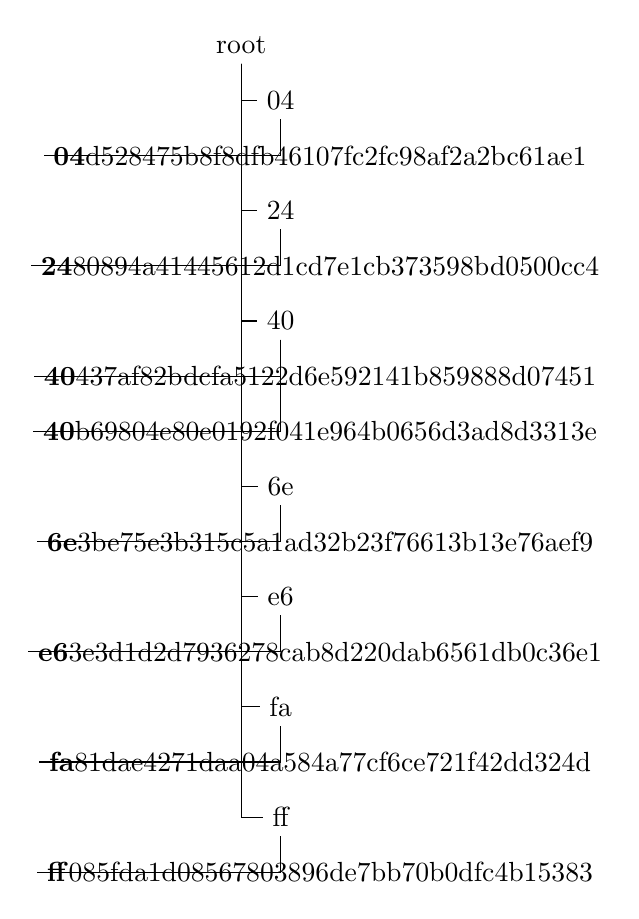
\begin{tikzpicture}[%
  grow via three points={one child at (0.5,-0.7) and
  two children at (0.5,-0.7) and (0.5,-1.4)},
  edge from parent path={(\tikzparentnode.south) |- (\tikzchildnode.west)}]
  \node {root}
    child { node {04}
      child { node {\textbf{04}d528475b8f8dfb46107fc2fc98af2a2bc61ae1}}
    }
    child [missing] {}
    child { node {24}
      child { node {\textbf{24}80894a41445612d1cd7e1cb373598bd0500cc4}}
    }
    child [missing] {}
    child { node {40}
      child { node {\textbf{40}437af82bdcfa5122d6e592141b859888d07451}}
      child { node {\textbf{40}b69804e80e0192f041e964b0656d3ad8d3313e}}
    }
    child [missing] {}
    child [missing] {}
    child { node {6e}
      child { node {\textbf{6e}3be75e3b315c5a1ad32b23f76613b13e76aef9}}
    }
    child [missing] {}
    child { node {e6}
      child { node {\textbf{e6}3e3d1d2d7936278cab8d220dab6561db0c36e1}}
    }
    child [missing] {}
    child { node {fa}
      child { node {\textbf{fa}81dae4271daa04a584a77cf6ce721f42dd324d}}
    }
    child [missing] {}
    child { node {ff}
      child { node {\textbf{ff}085fda1d08567803896de7bb70b0dfc4b15383}}
    };

\end{tikzpicture}
\tikzstyle{every node}=[]